\documentclass[xcolor={dvipsnames}]{beamer} % dvipsnames gives more built-in colors
\mode<presentation>

\usetheme{Boadilla}

\definecolor{GWdarkblue}{HTML}{033C5A}

\usecolortheme[named=GWdarkblue]{structure}

% Sets the font
\usepackage[defaultfam,tabular,lining]{montserrat}
% Capital case titles
\setbeamerfont{title}{shape=\scshape}
\setbeamerfont{frametitle}{shape=\scshape}

%Remove "Figure" from captions
\setbeamertemplate{caption}{\raggedright\insertcaption\par}

\usepackage{graphicx}
\usepackage{hyperref}

\title[Wrapping Up]{Wrapping Up}
\author[SMPA 2152]{Data Analysis for Journalism and Political Communication (Fall 2024)}
\date{Prof. Bell}

\begin{document}

%%%%%%%%%%%%%%%%%%%%%%%%%%%%%%%%%%%%%%%%%%%%%%%%%%%%%%%%%%%%%%%%%%
\frame{
    \titlepage
}

%%%%%%%%%%%%%%%%%%%%%%%%%%%%%%%%%%%%%%%%%%%%%%%%%%%%%%%%%%%%%%%%%%
\frame{
    \frametitle{Think-Pair-Share}
    \begin{enumerate}
        \item What are the most important ideas that you will take away from this class?
        \item What burning questions do you still have about data analysis?
    \end{enumerate}
}

%%%%%%%%%%%%%%%%%%%%%%%%%%%%%%%%%%%%%%%%%%%%%%%%%%%%%%%%%%%%%%%%%%
\frame{
    \frametitle{Chalabi: 3 Ways to Spot a Bad Statistic}
    \centering
    \href{https://www.ted.com/talks/mona_chalabi_3_ways_to_spot_a_bad_statistic}{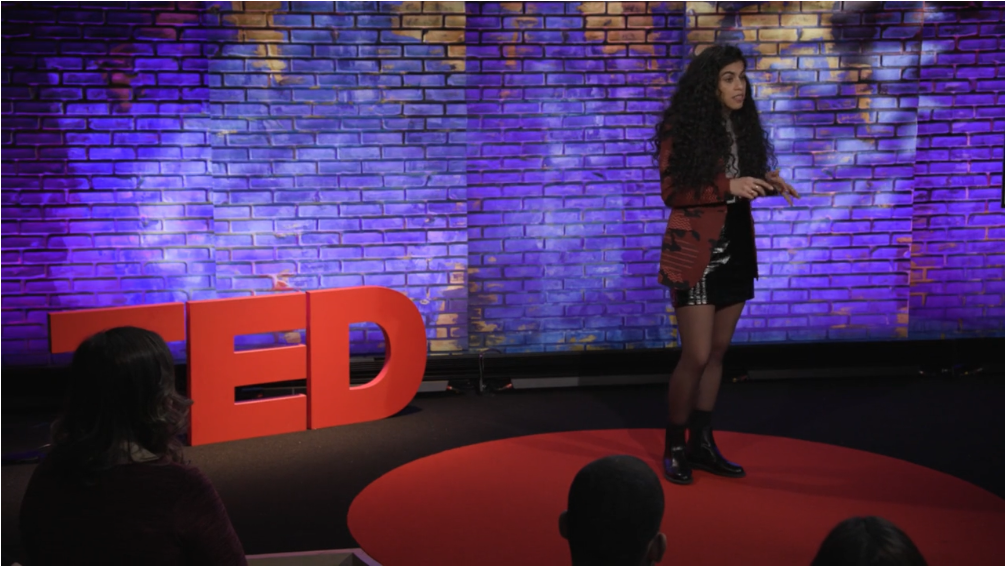
\includegraphics[height = .6\textheight]{chalabi-ted-talk.png}}
    
    \begin{enumerate}
        \item Can you see uncertainty?
        \item Can we look beyond the averages?
        \item How was the data collected?
    \end{enumerate}
}

%%%%%%%%%%%%%%%%%%%%%%%%%%%%%%%%%%%%%%%%%%%%%%%%%%%%%%%%%%%%%%%%%%
\frame{
    \frametitle{Can you see the uncertainty?}
    \begin{itemize}[<+->]
        \item Whenever we take a sample and try to make inferences about a population, there is uncertainty
        \only<1>{
            ~\\~\\
            \centering
            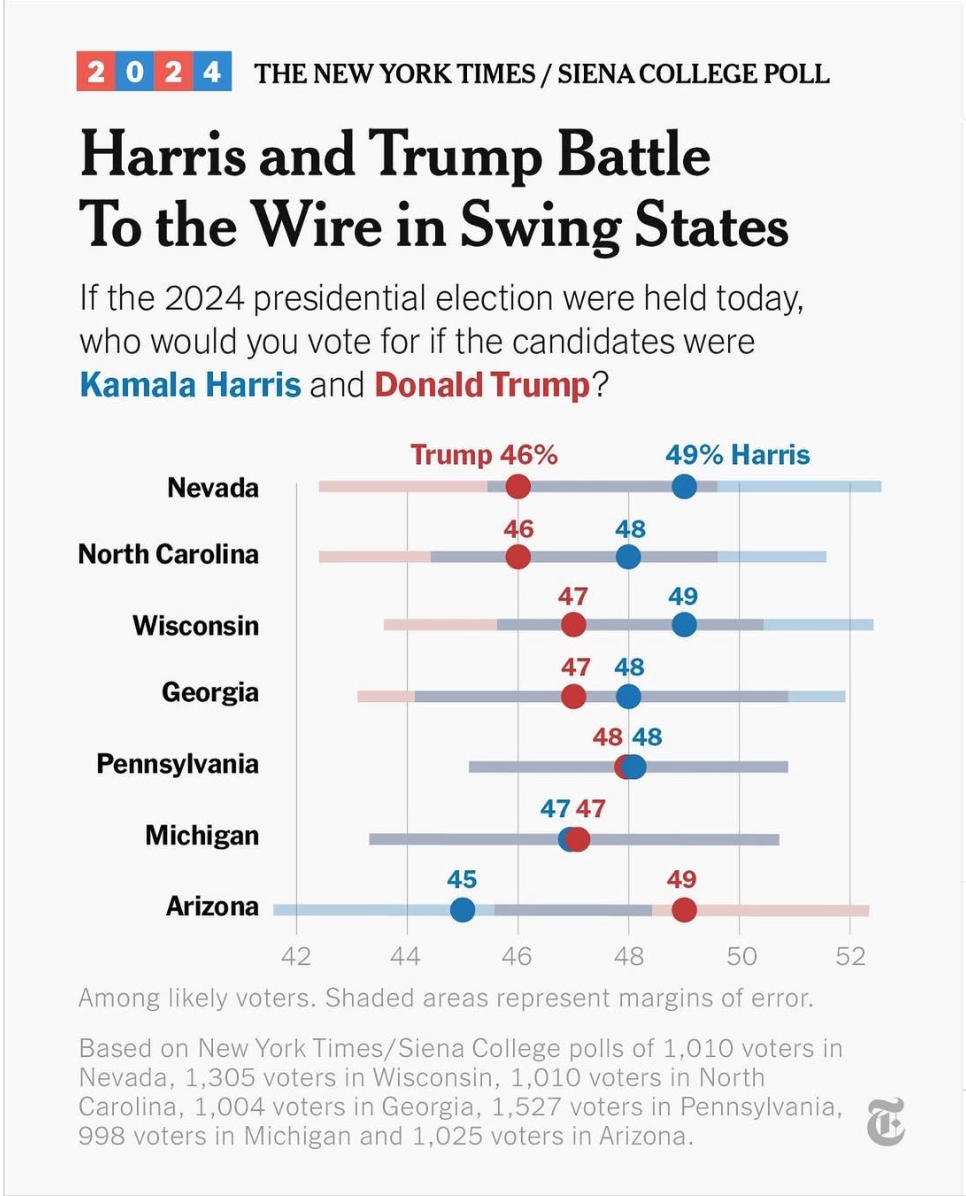
\includegraphics[height = .6\textheight]{nyt_final_polls.png}
            }
        \item There is also uncertainty when making causal claims
        \only<2>{
            ~\\~\\
            \centering
            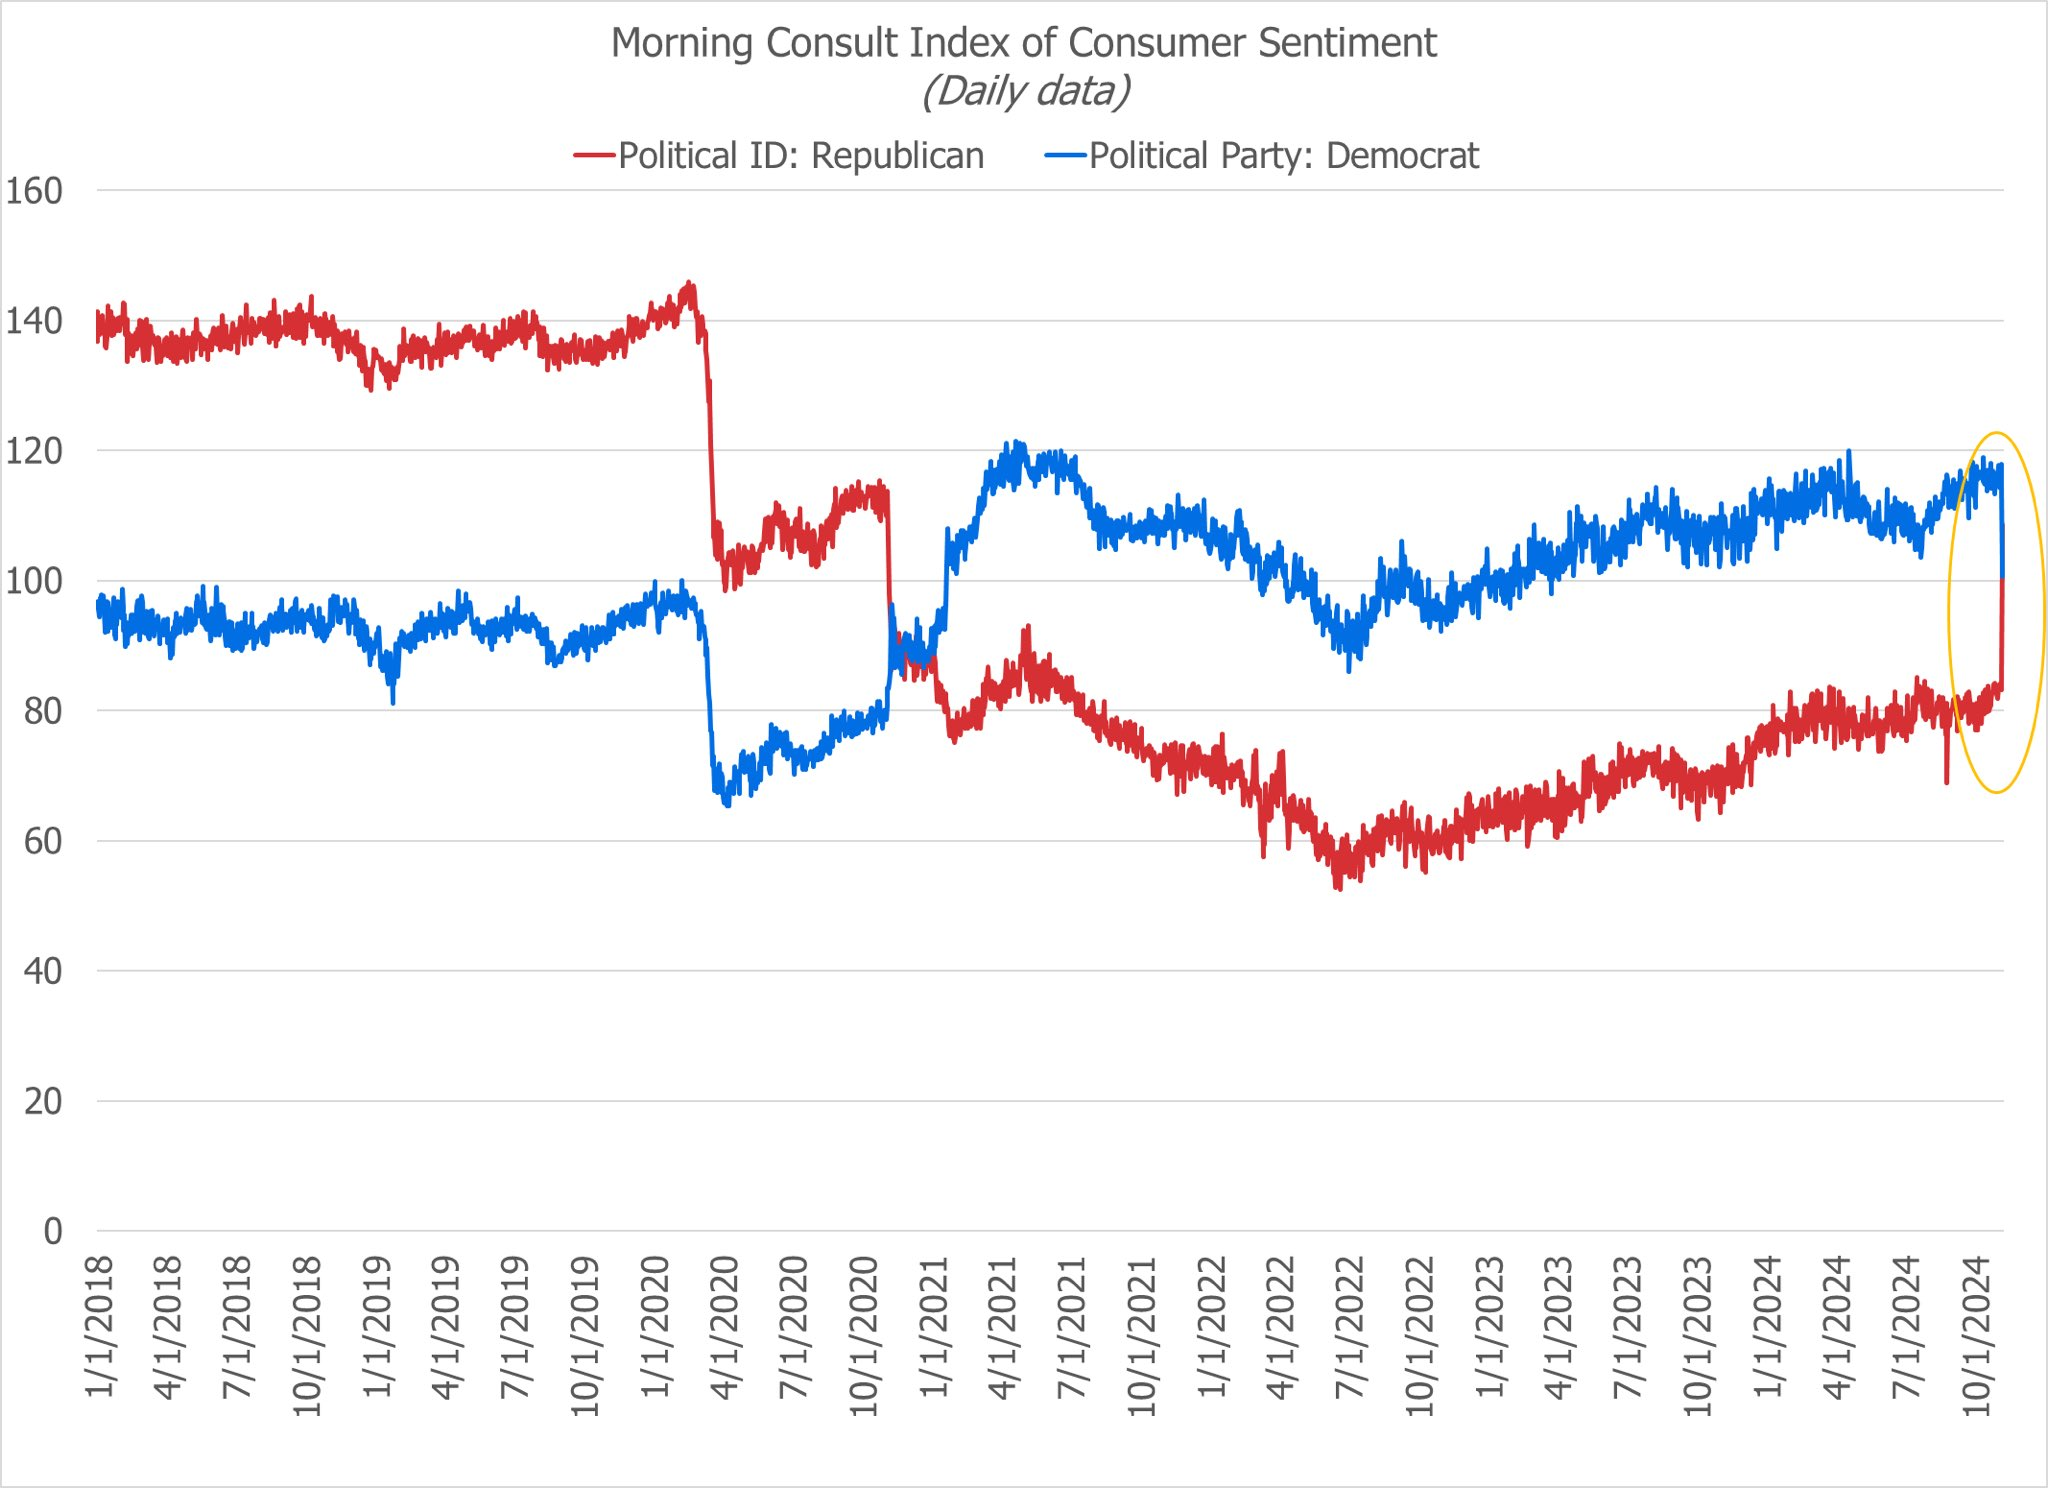
\includegraphics[height = .6\textheight]{consumer_sentiment.jpeg}
            }
    \end{itemize}
}

%%%%%%%%%%%%%%%%%%%%%%%%%%%%%%%%%%%%%%%%%%%%%%%%%%%%%%%%%%%%%%%%%%
\frame{
    \frametitle{Can we look beyond the averages?}
    \begin{itemize}[<+->]
        \item We have to be conscious of \href{https://x.com/rp_griffin/status/1857414569628475691}{researcher degrees of freedom}.
        \item There is both a science and an art to accurately communicating about data using data visualizations.
        ~\\~\\
            \centering
            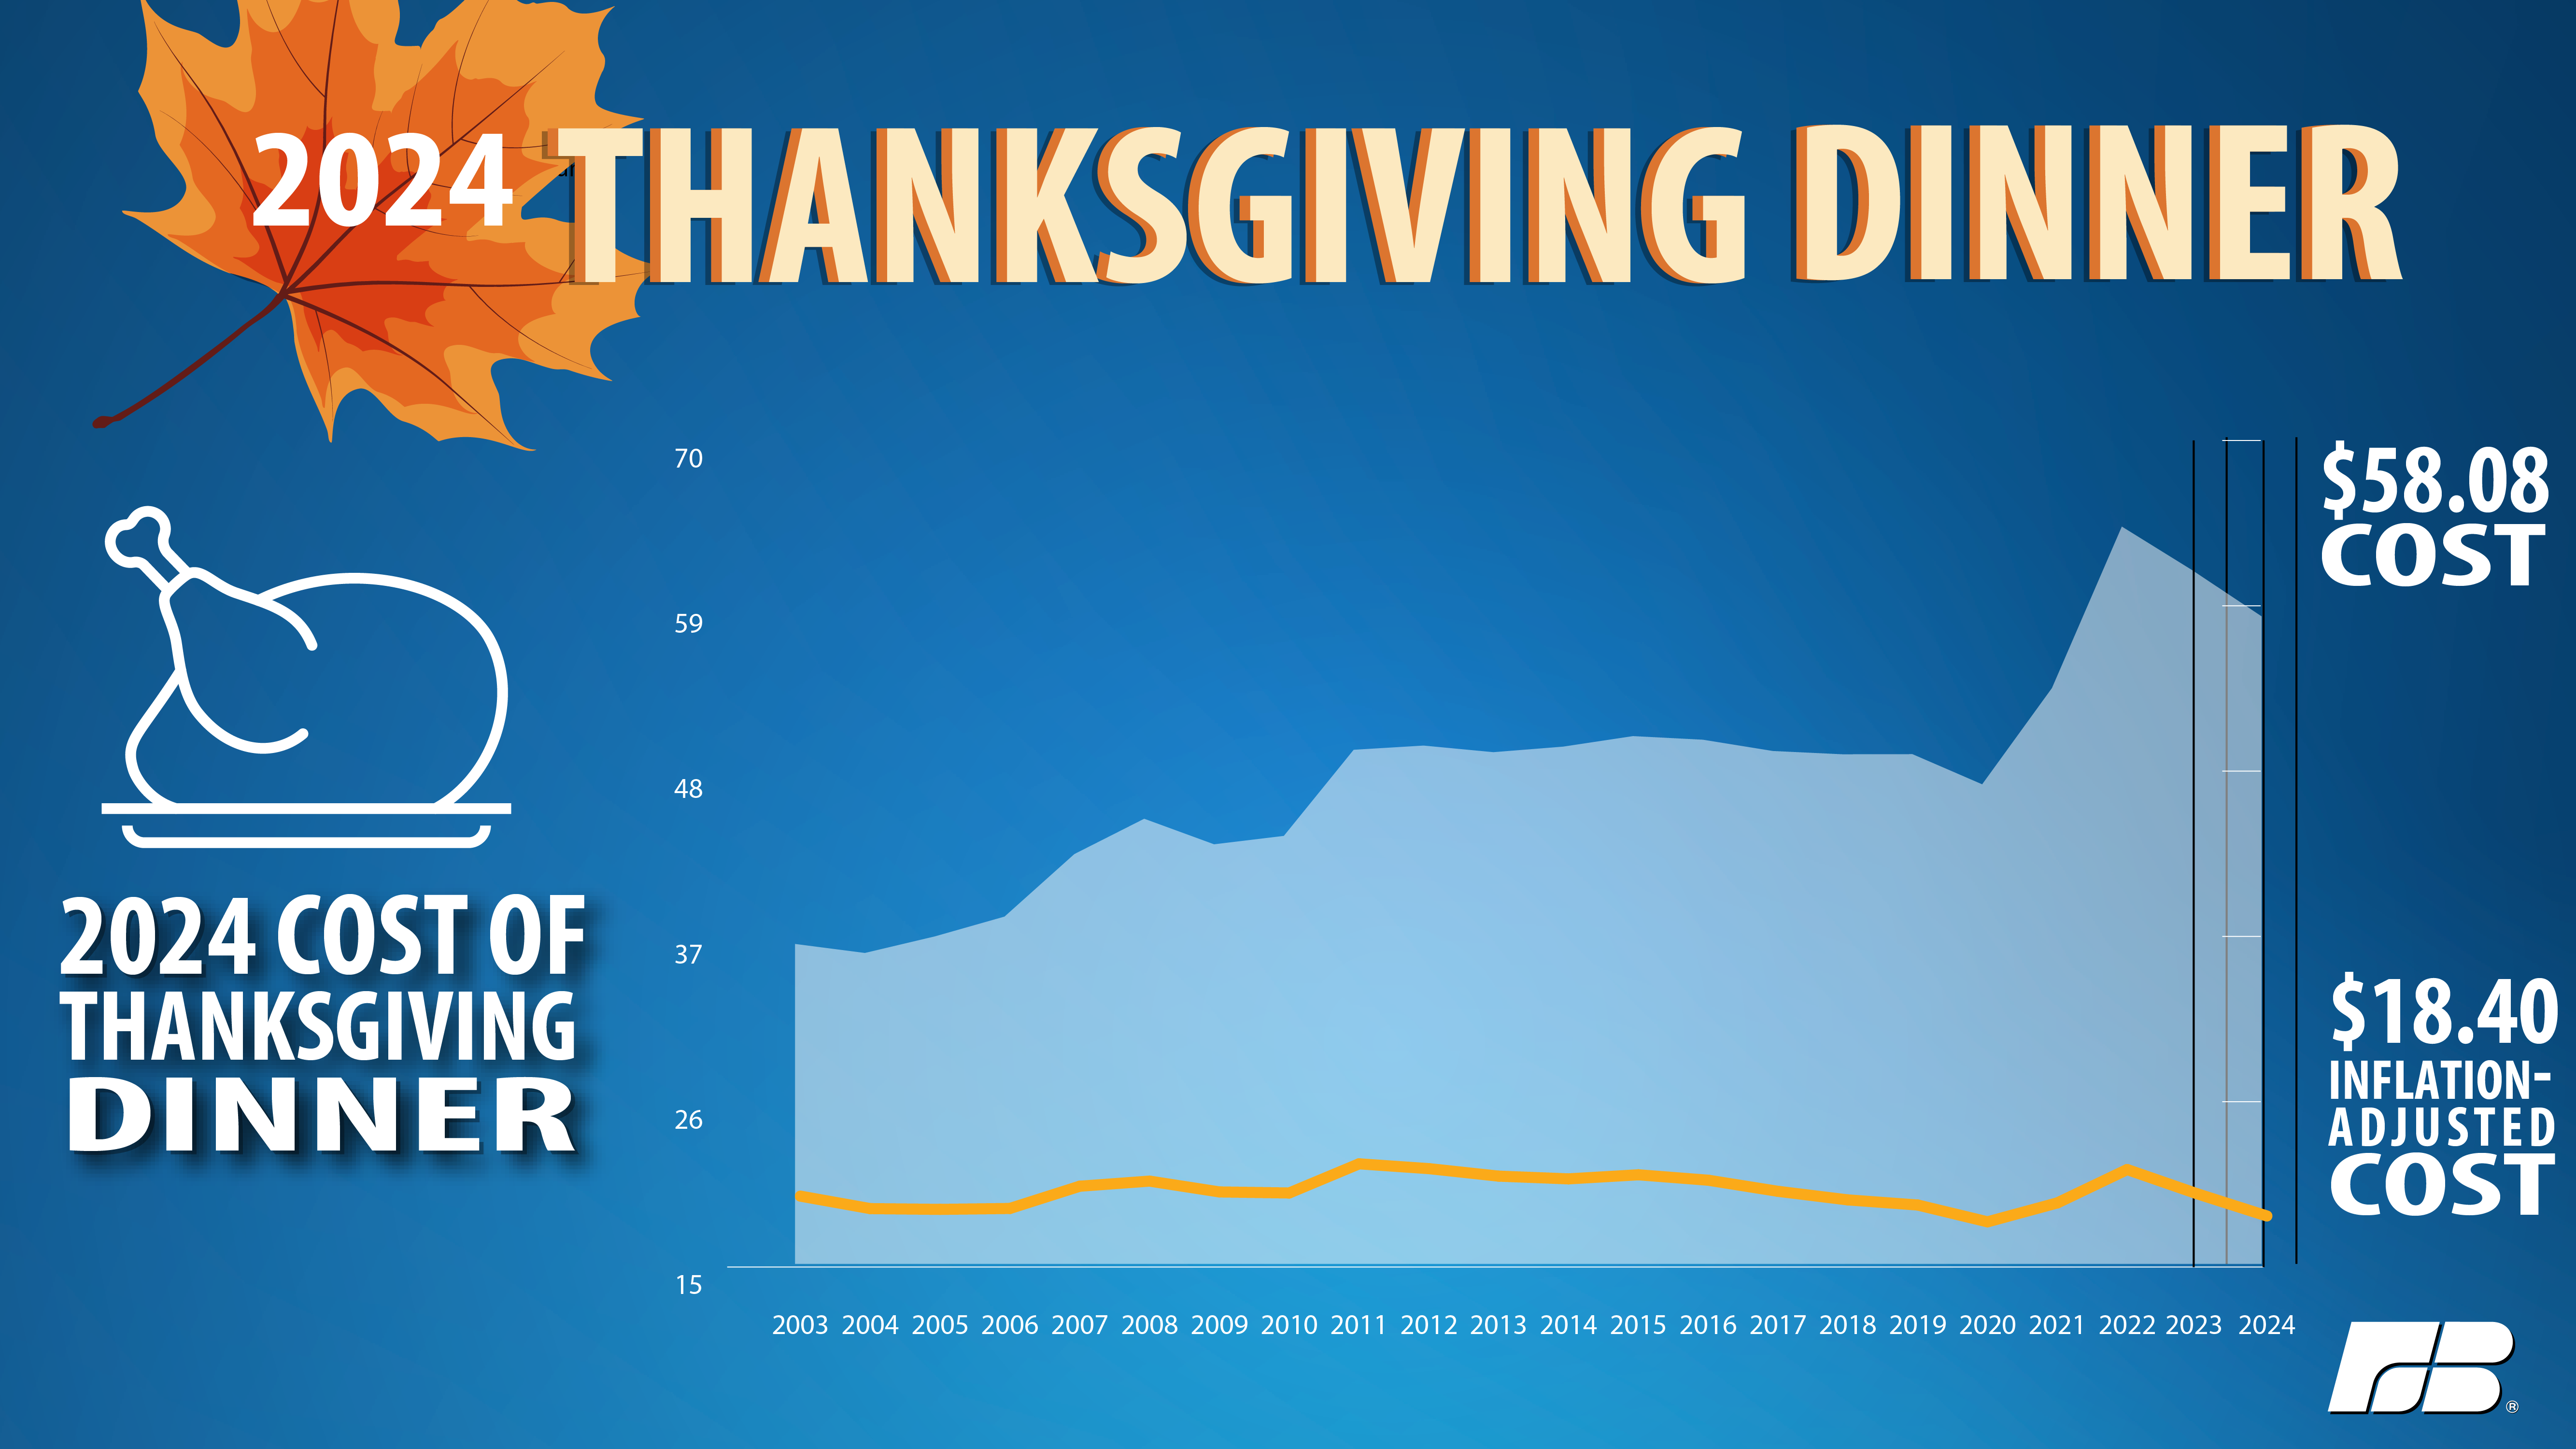
\includegraphics[height = .5\textheight]{2024_thanksgiving_dinner.png}
    \end{itemize}
}

%%%%%%%%%%%%%%%%%%%%%%%%%%%%%%%%%%%%%%%%%%%%%%%%%%%%%%%%%%%%%%%%%%
\frame{
    \frametitle{How was the data collected?}
    \only<1> {
        \centering
        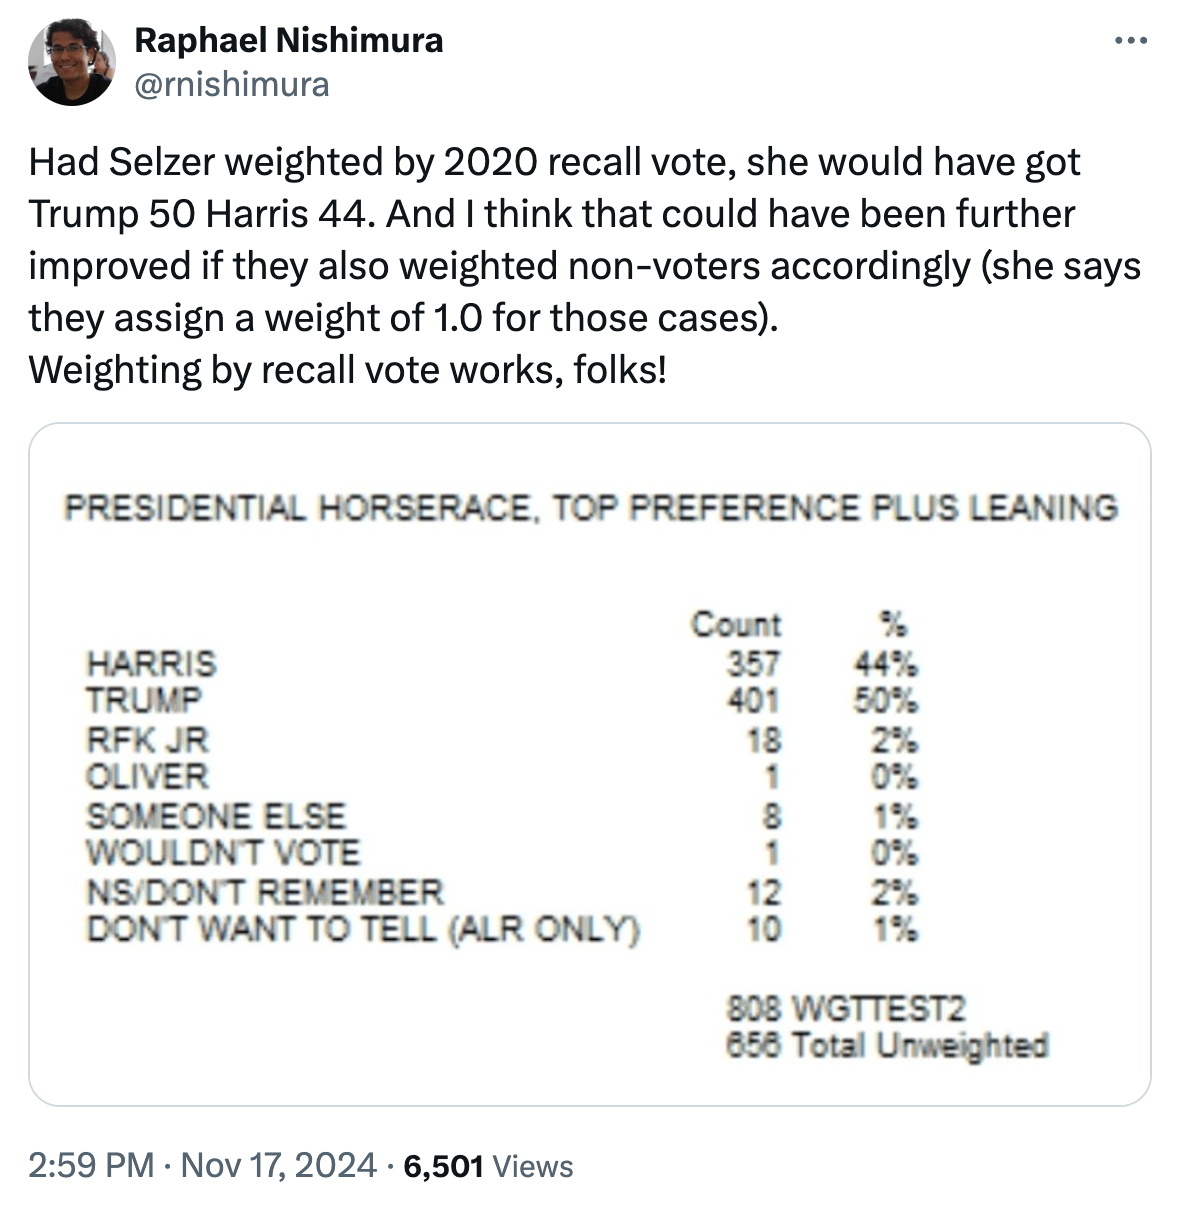
\includegraphics[height = .8\textheight]{selzer.png}
    }
    \only<2> {
        \centering
        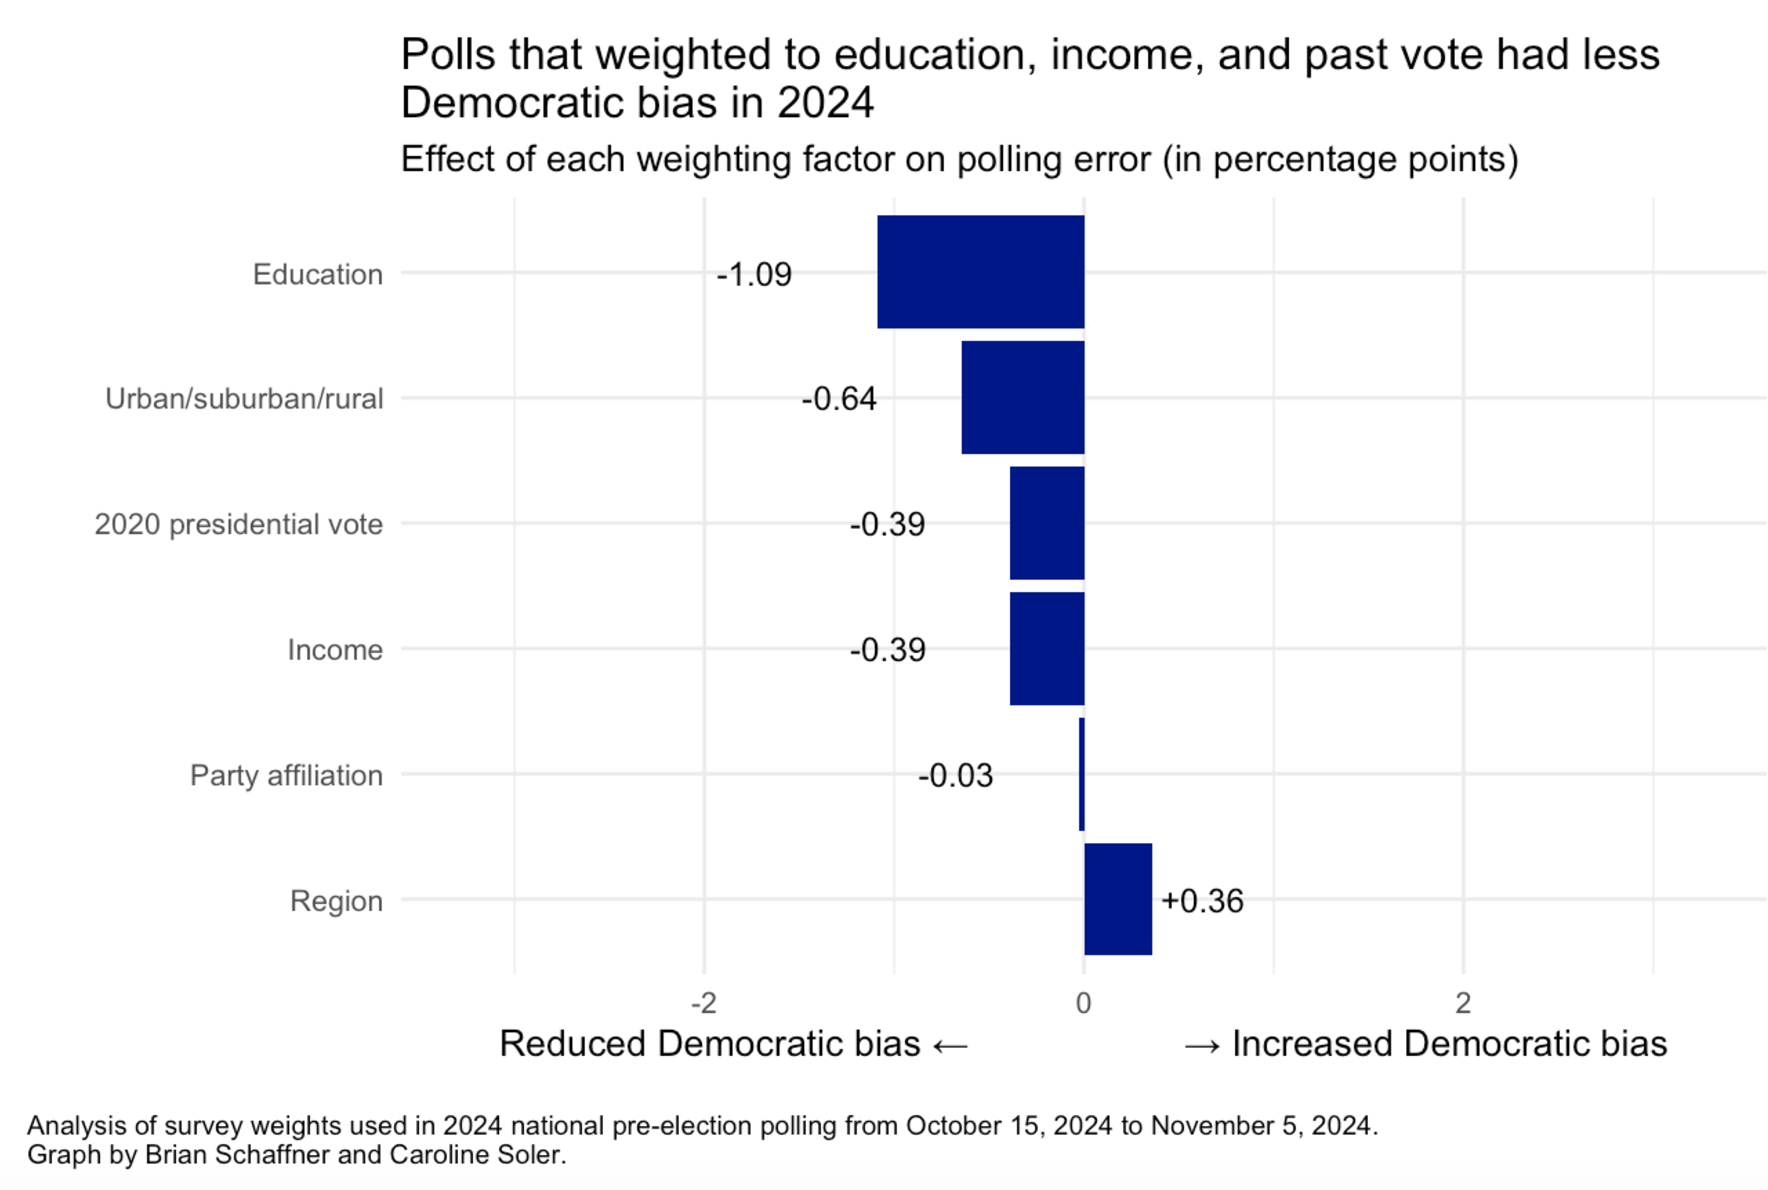
\includegraphics[height = .8\textheight]{weighting_2024.png}
    }
    \only<3> {
        \centering
        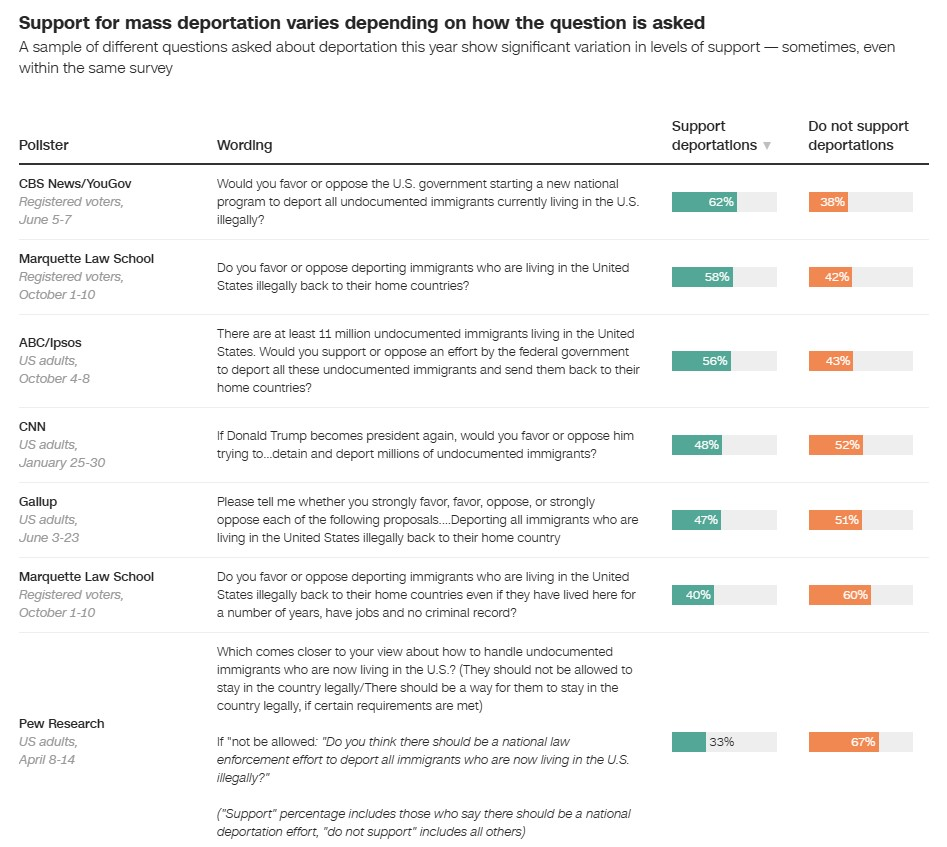
\includegraphics[height = .8\textheight]{poll_questions.jpeg}
    }
}

%%%%%%%%%%%%%%%%%%%%%%%%%%%%%%%%%%%%%%%%%%%%%%%%%%%%%%%%%%%%%%%%%%
\frame{
    \frametitle{You Learned R!}
    \begin{columns}
    \begin{column}{0.5\textwidth}
       \begin{itemize}
            \item Make charts for 3+ variables
            \item Load data
            \item Filter data
            \item Create and change data
            \item Summarize data
            \item Pivot data (tidy data)
            \item Join data
       \end{itemize}
    \end{column}
    \begin{column}{0.5\textwidth}  %%<--- here
        \begin{itemize}
            \item Work with dates
            \item Work with strings
            \item Work with factors
            \item Analyze poll data
            \item Make maps
            \item Conduct t-tests
            \item Run regressions
            \item Create reports
       \end{itemize}
    \end{column}
    \end{columns}
}


%%%%%%%%%%%%%%%%%%%%%%%%%%%%%%%%%%%%%%%%%%%%%%%%%%%%%%%%%%%%%%%%%%
\frame{
    \frametitle{How Did the Polls Do in 2024?}
    \only<1> {
        \centering
        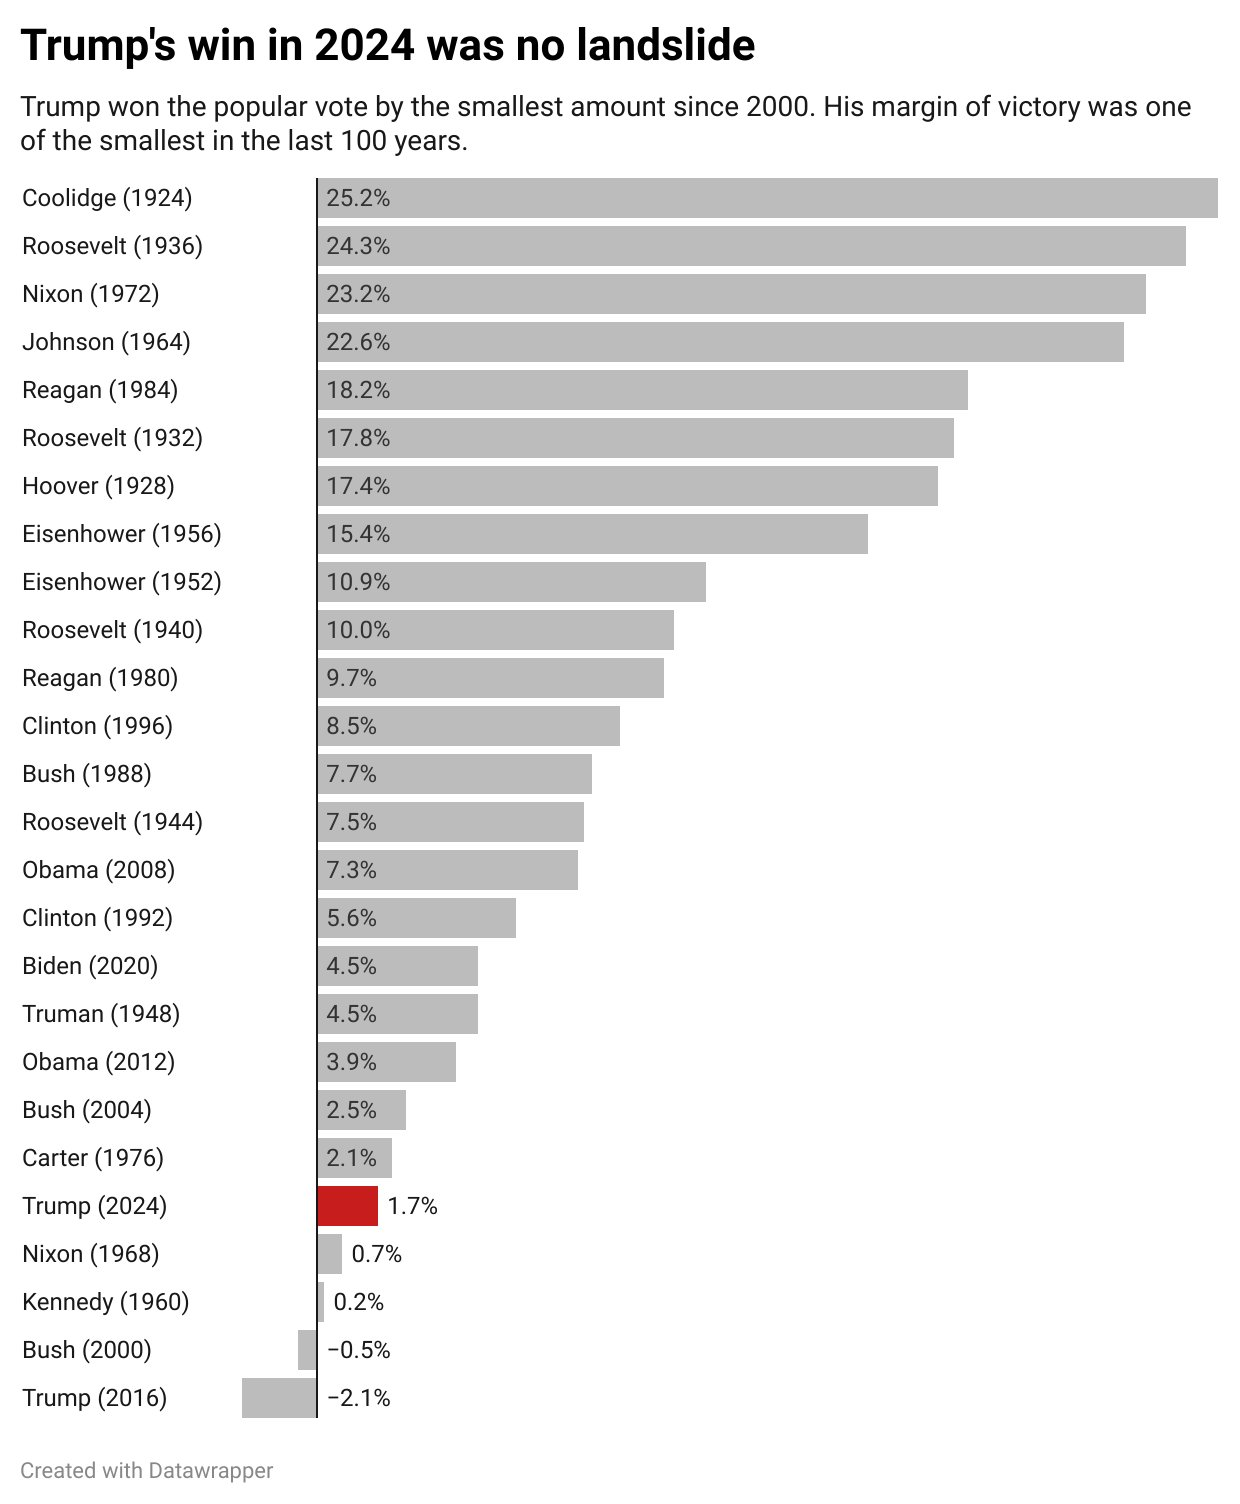
\includegraphics[height = .8\textheight]{close_election.jpeg}
    }
    \only<2> {
        \centering
        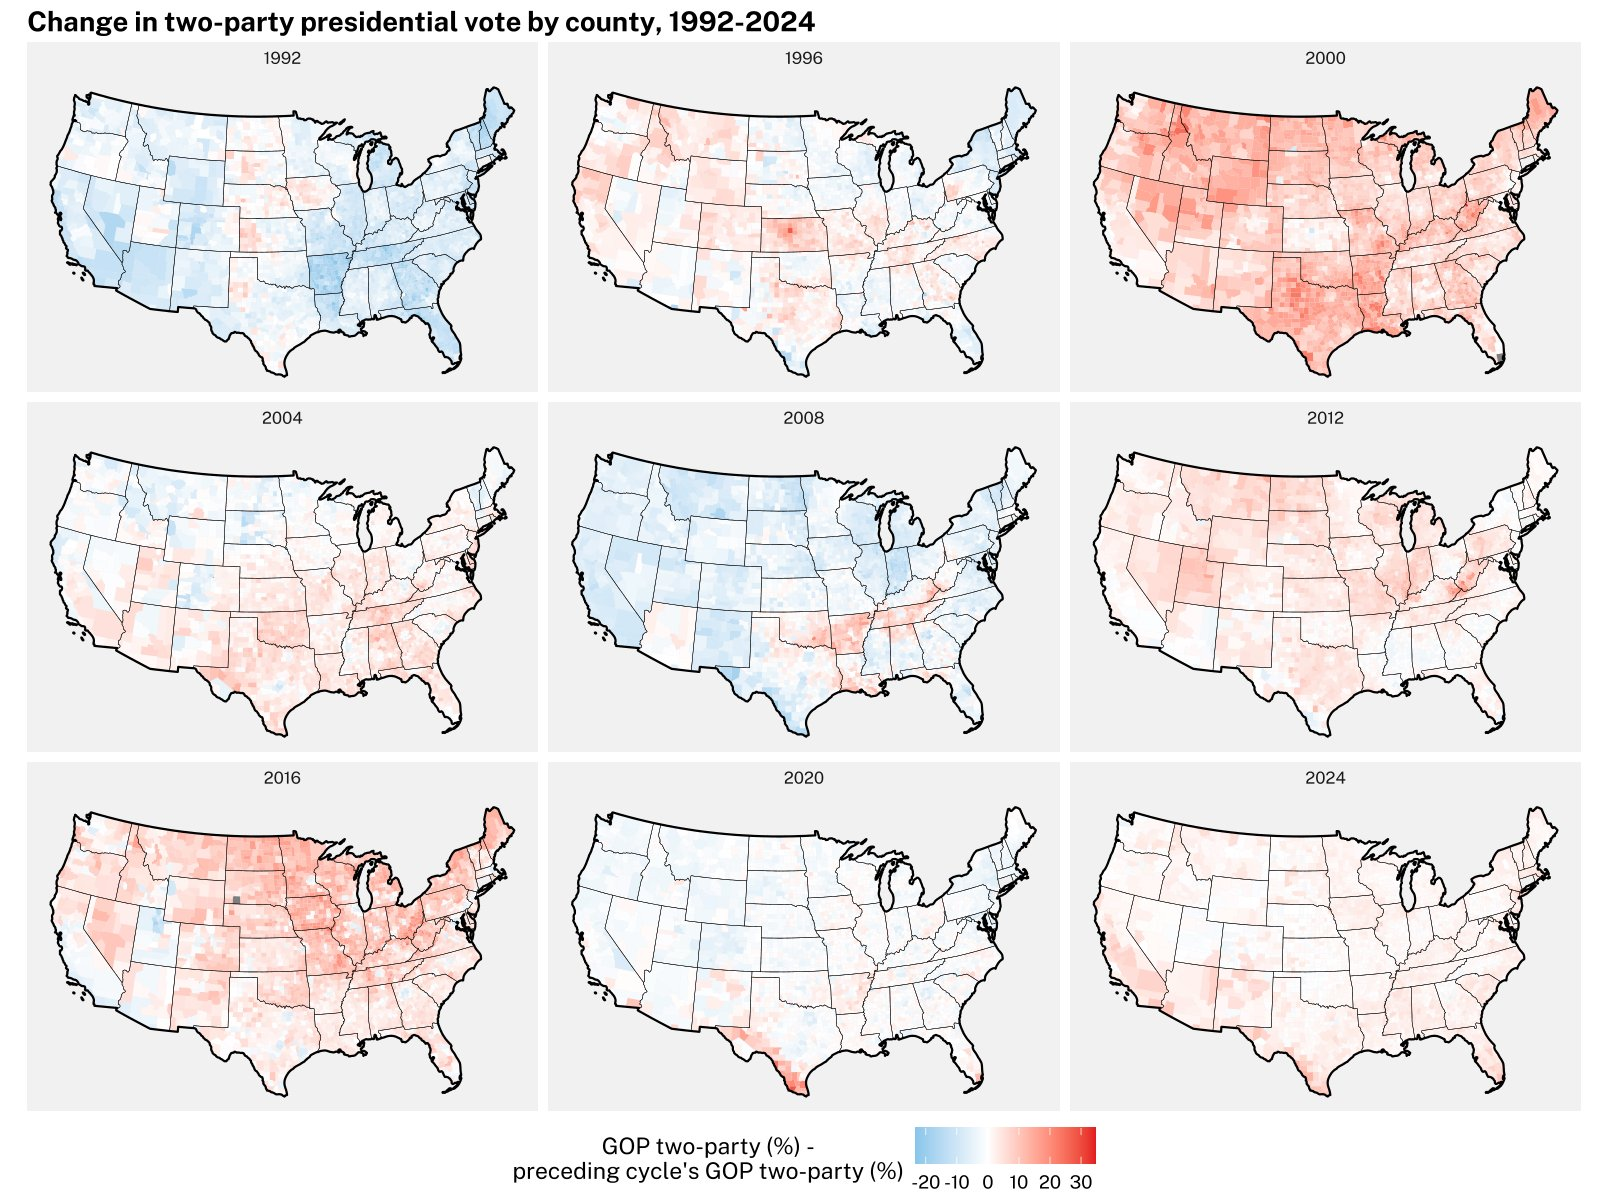
\includegraphics[height = .8\textheight]{vote_shift.jpeg}
    }
    \only<3> {
        \centering
        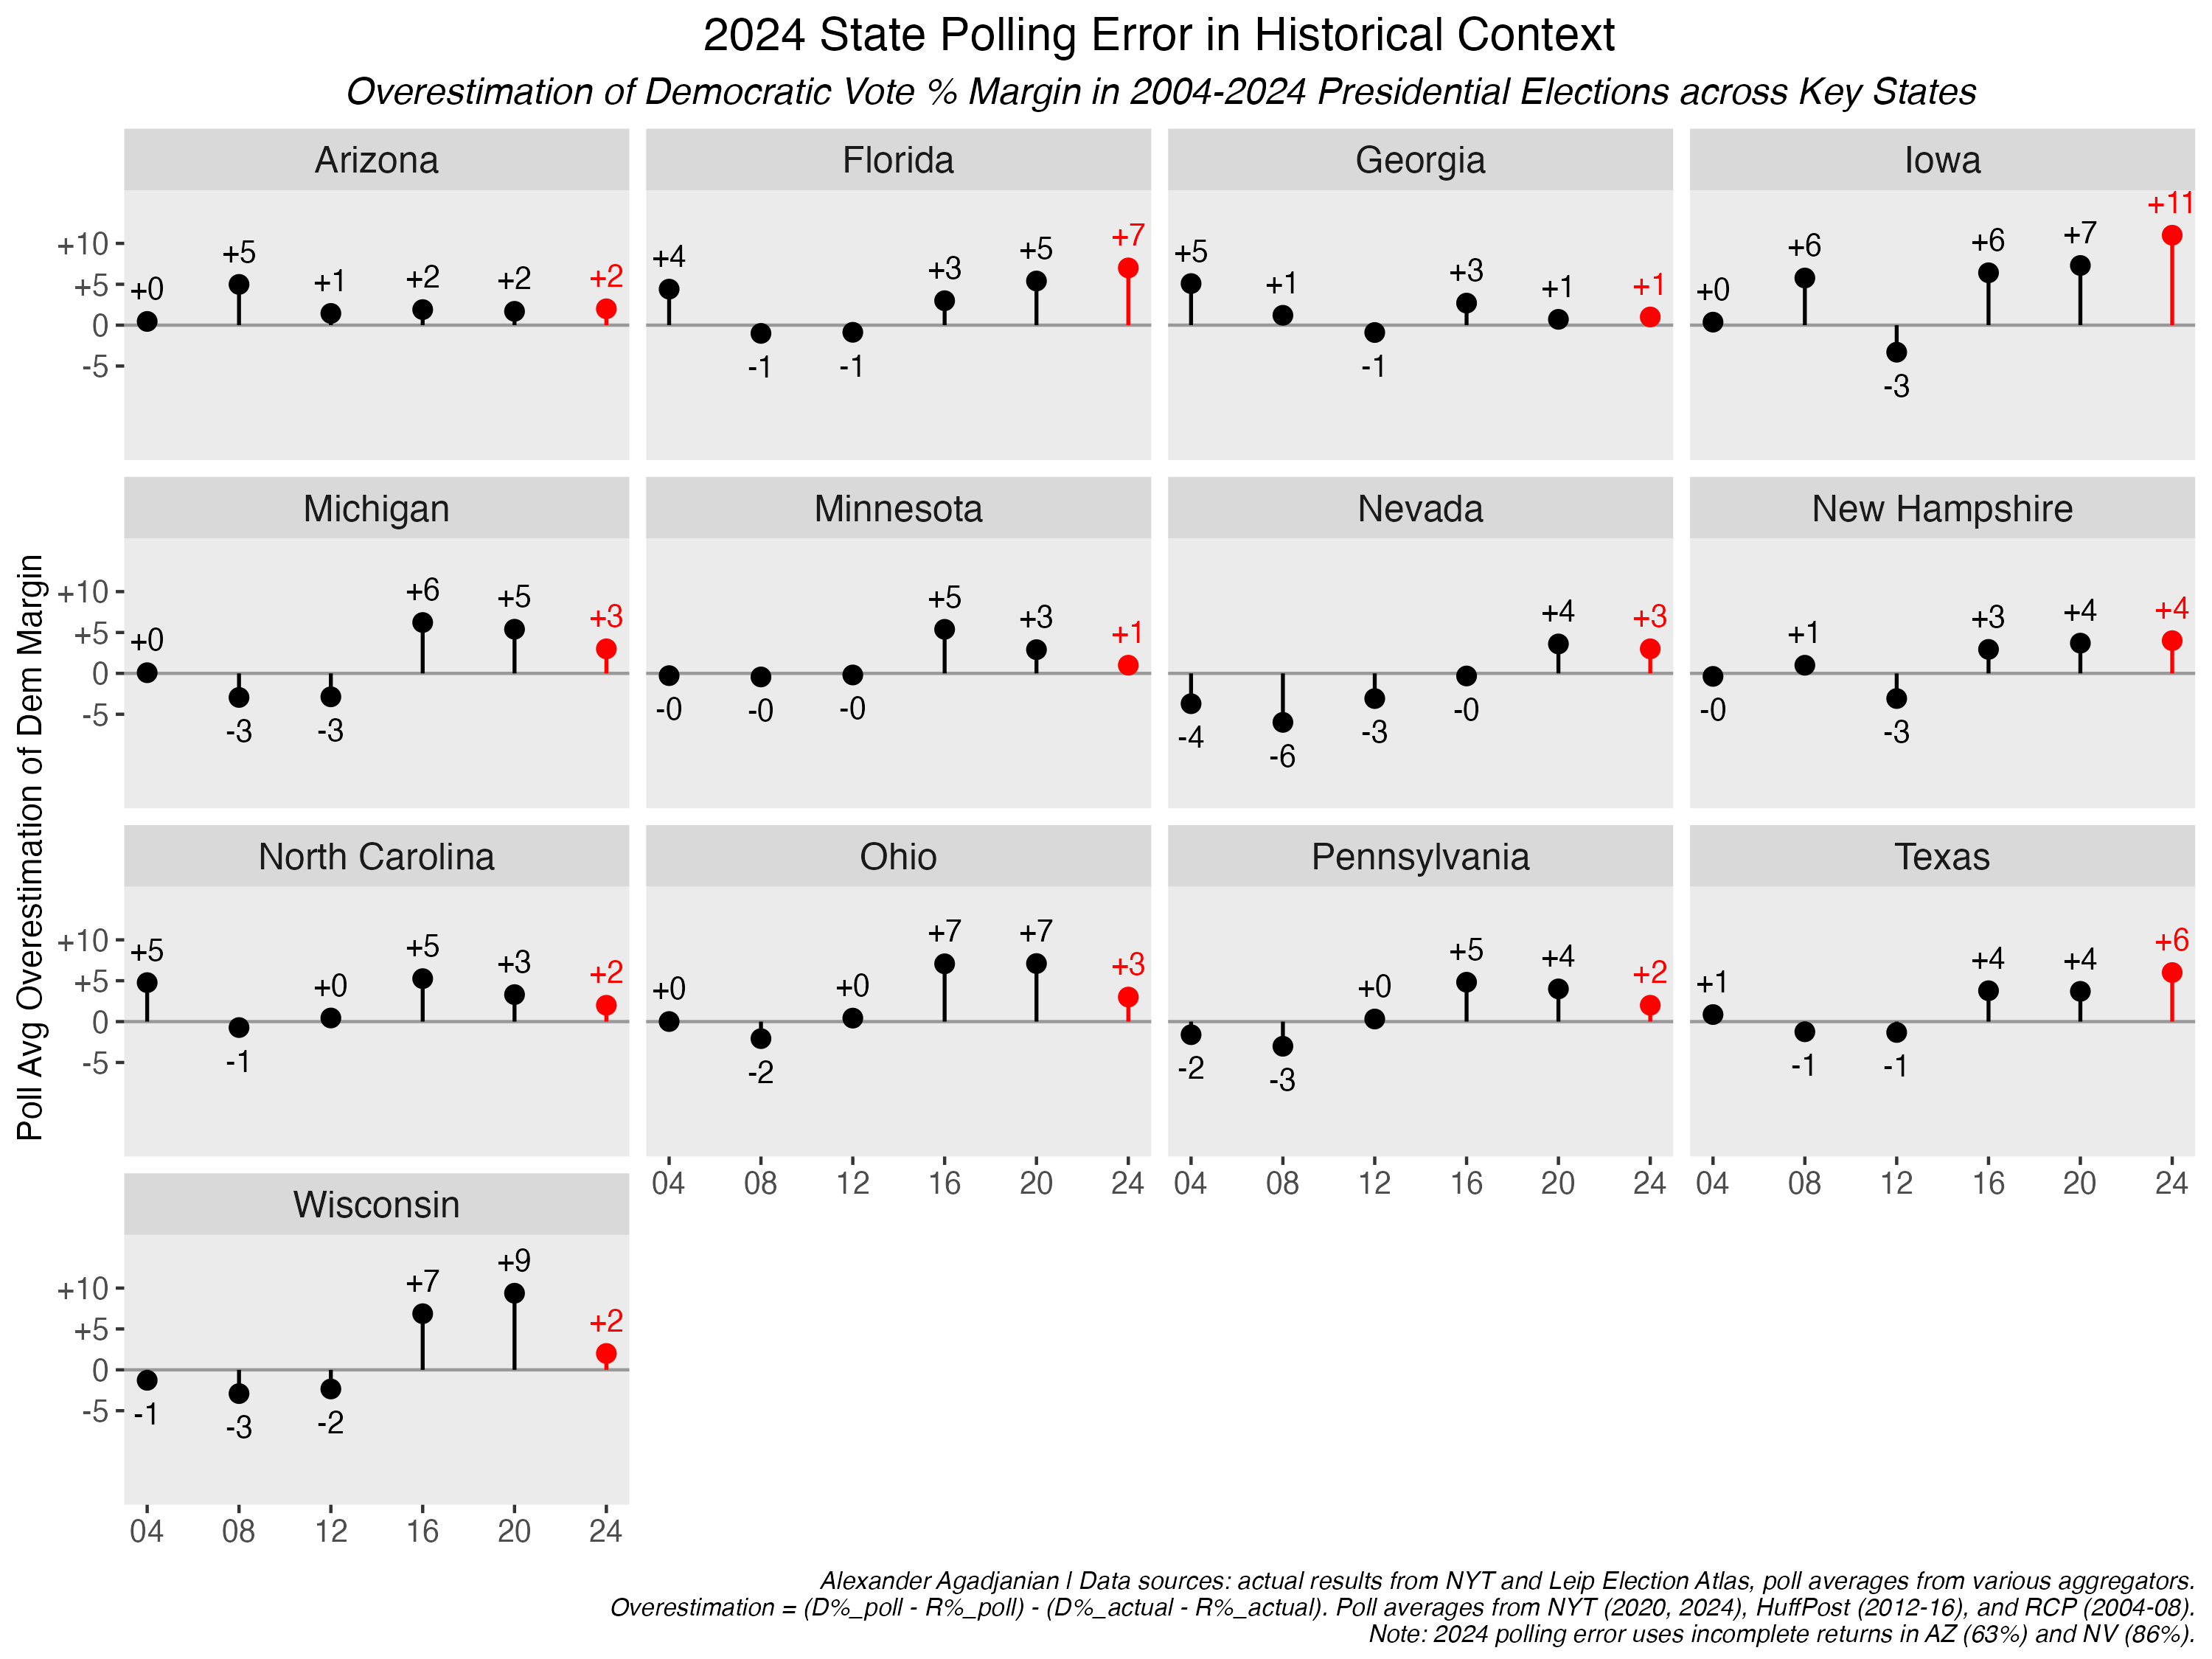
\includegraphics[height = .8\textheight]{state_polling_misses.png}
    }
    \only<4> {
        \centering
        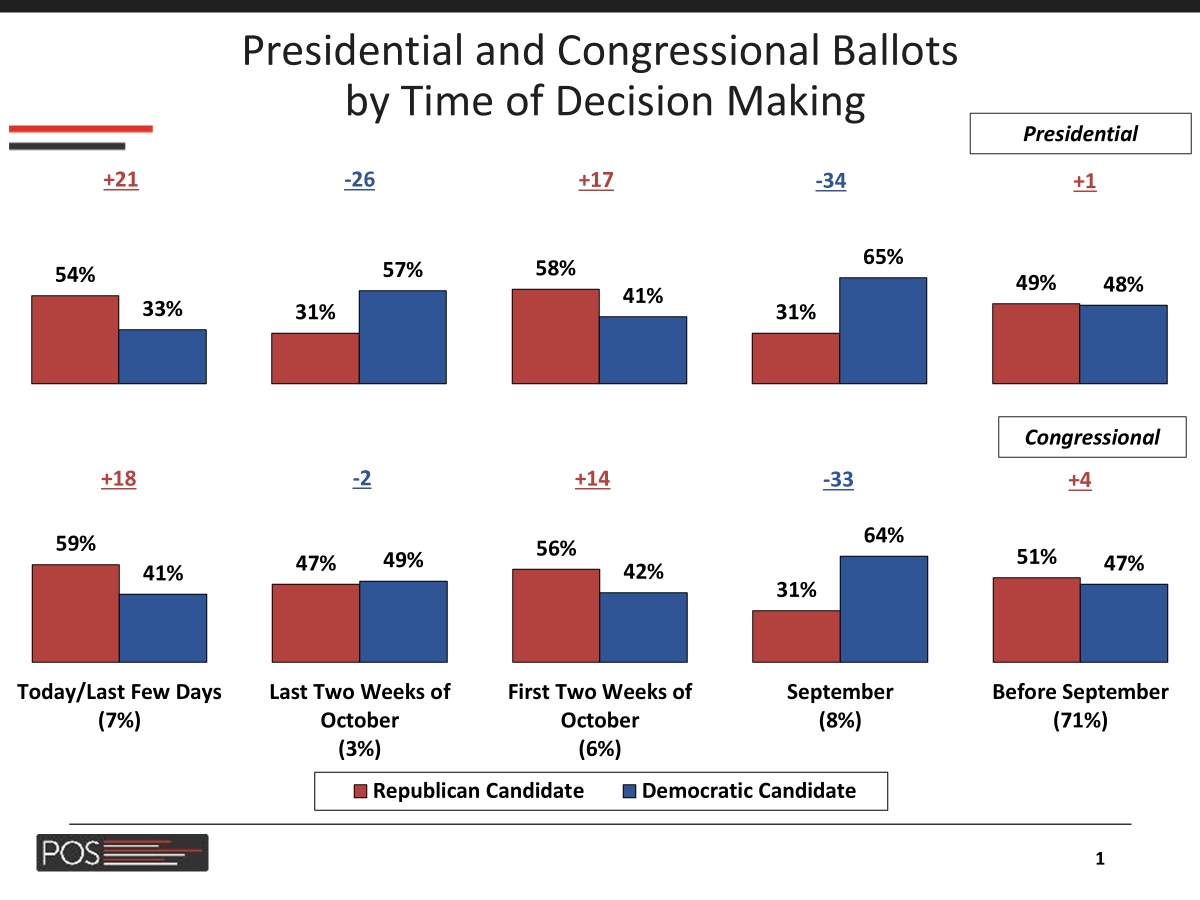
\includegraphics[height = .8\textheight]{late_deciders.png}
    }
    \only<5> {
        \centering
        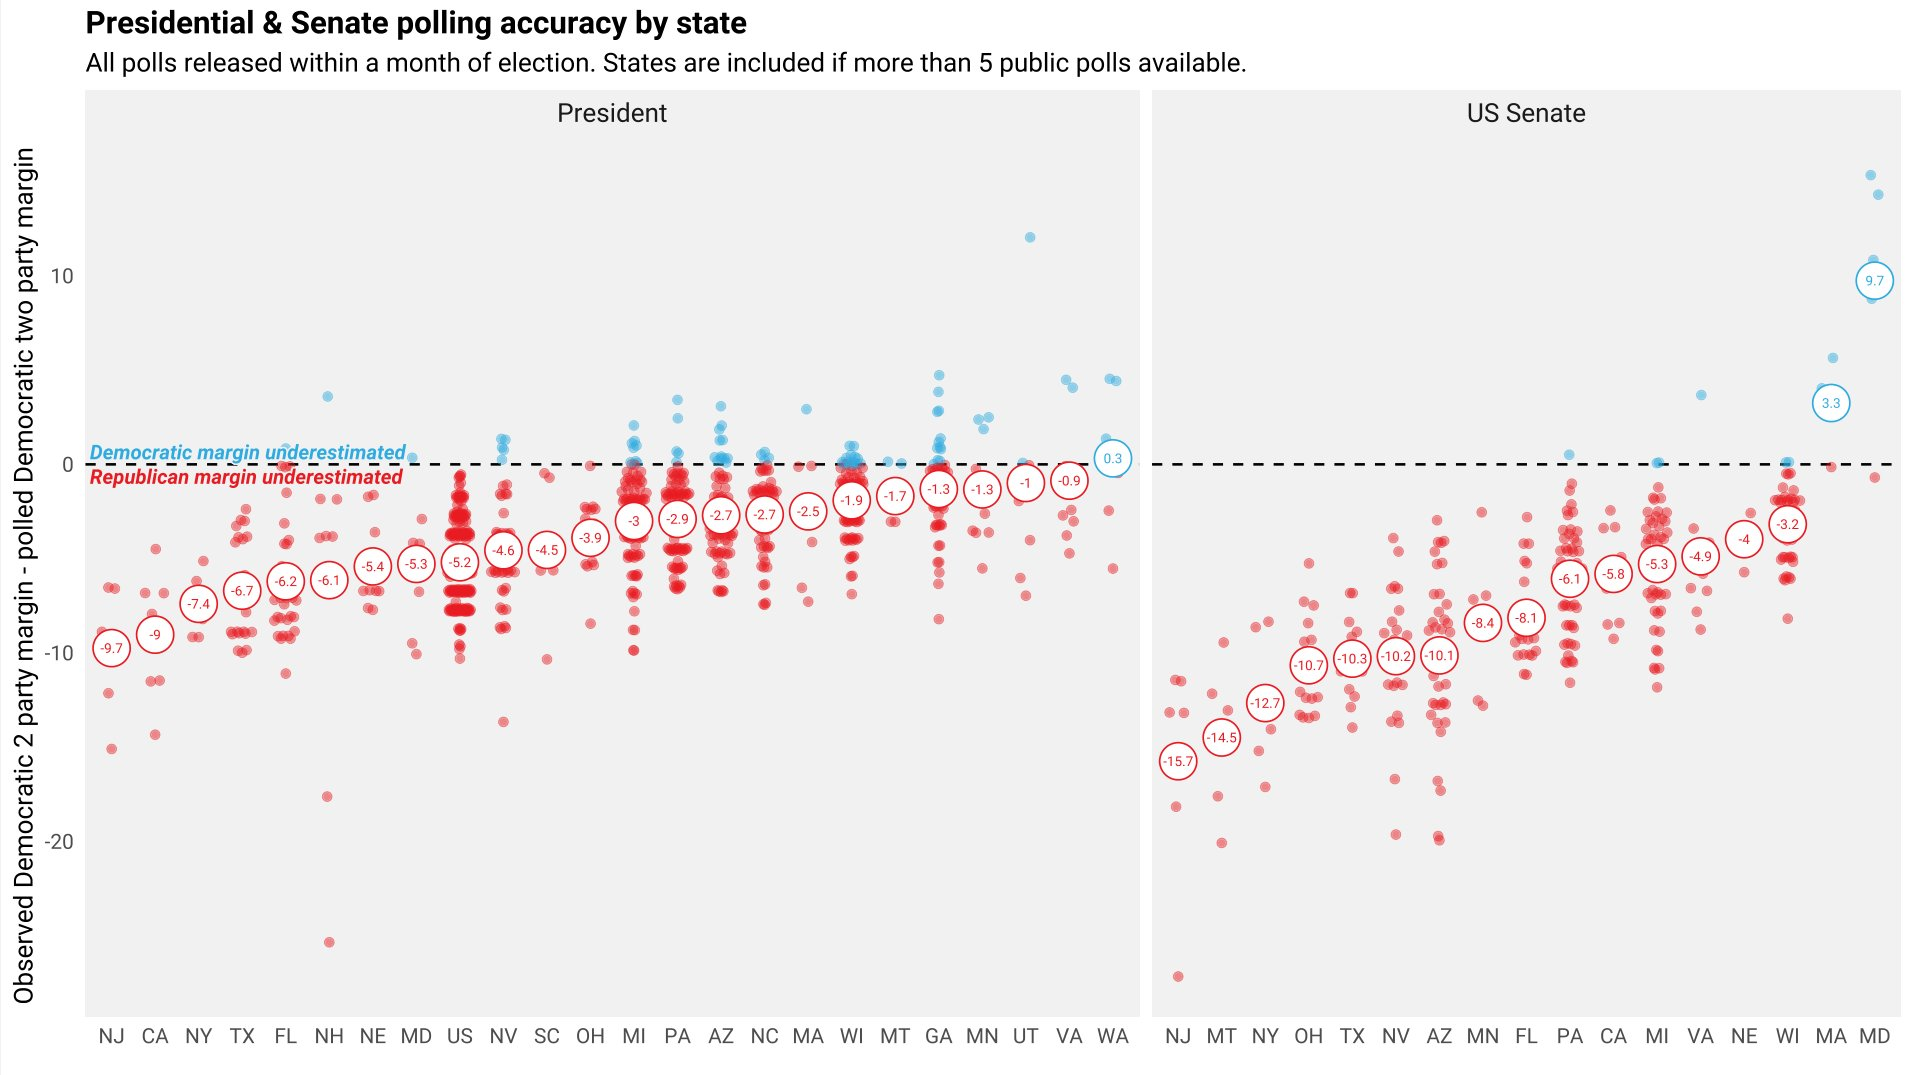
\includegraphics[width = .9\textwidth]{direction_of_miss.jpeg}
    }
}

\end{document}
